\begin{quote} ``We are drowning in information, while starving for wisdom'' - \textit{E.O. Wilson} \end{quote}

The most fundamental unit of life, a living cell, functions by a complex orchestration of various genes and their products (\acs{mRNA}, proteins etc.). In a more abstract manner we can say that genes are interrelated in highly structured networks of information flow in order for the cells to function. A network of such gene products (proteins) known as \acp{TF} which regulate the production of other transcription factors or other proteins is called a \acfi{TRN} or \acfi{GRN}. The understanding and reconstruction of this regulation process at a global level is one of the major challenges for the nascent field of bio-informatics \citep{kernel_methodsvert2004}. 

Considerable work has been done by molecular biologists over the past many years in identifying the functions of specific genes. In an ideal world it would be desirable to apply these results in order to build detailed models of regulation where the precise action of each gene is understood. However, the large number of genes and the complexity of the regulation process means that this approach has not been feasible. Research into discovering causal models based on the actions of individual genes has encountered a major difficulty in estimating a large number of parameters from a paucity of experimental data. Fortunately however, biological organisation opens up the possibility of modelling at a less detailed level. In nature, complex functions of living cells are carried out through the concerted activities of many genes and gene products which are organized into co-regulated sets also known as \textit{regulatory modules} \citep{segal03module}. Understanding the organization of these sets of genes will provide insights into the cellular response mechanism under various conditions. 

Recent advances in measurement technologies and computing resources have led to the wide availability of a considerable volume of genome-wide data on gene activity measured using several diverse techniques. By fusing this data using an integrative approach, we can try to unravel the regulation process at a more global level. Although an integrated model could never be as precise as one built from a small number of genes in controlled conditions, such global modelling can provide insights into higher processes where many genes are working together to achieve a task. Various techniques from statistics, machine learning and computer science have been employed by researchers for the analysis and combination of the different types of data in an attempt to identify and understand the function of regulatory modules. 

There are two underlying problems resulting from the nature of the available data. Firstly, each of the different data types (microarray, DNA-binding, protein-protein interaction and sequence data) provides a partial and noisy picture of the regulatory process. They need to be integrated in order to obtain an improved and reliable picture of the whole underlying process. Secondly, the amount of data that is available from each of these techniques is severely limited. To learn good models we need lots of data \citep{yeung04fromexpr}, yet data is only available for a few experiments of each type. To alleviate this problem many researchers have taken the path of merging all available datasets before carrying out an analysis. Thus there can be some confusion regarding the term \textit{integrative} because it has been used to describe both of these two very different approaches to data integration: one among datasets of the same type, for example microarrays, but from different experiments, and the other among different types of data, for example microarray and DNA binding data. The goal of this thesis is to analyze the problems resulting from the existing integrative approaches and suggest better solutions for improved data integration.

\section{Biological Background}
This section presents a brief overview of elementary molecular biology concepts that are essential in order to fully understand this thesis. For a detailed understanding please refer to any standard text on molecular biology like \citet{alberts02molecular}\footnote{a free web book is available at \url{http://www.web-books.com/MoBio/}}; \citet{hunter_molbio93} has written a brief yet excellent introduction specially for people with computing background.

\begin{figure}
 \parbox[b]{0.5 \textwidth}{
 \begin{center}
 \scalebox{0.50}{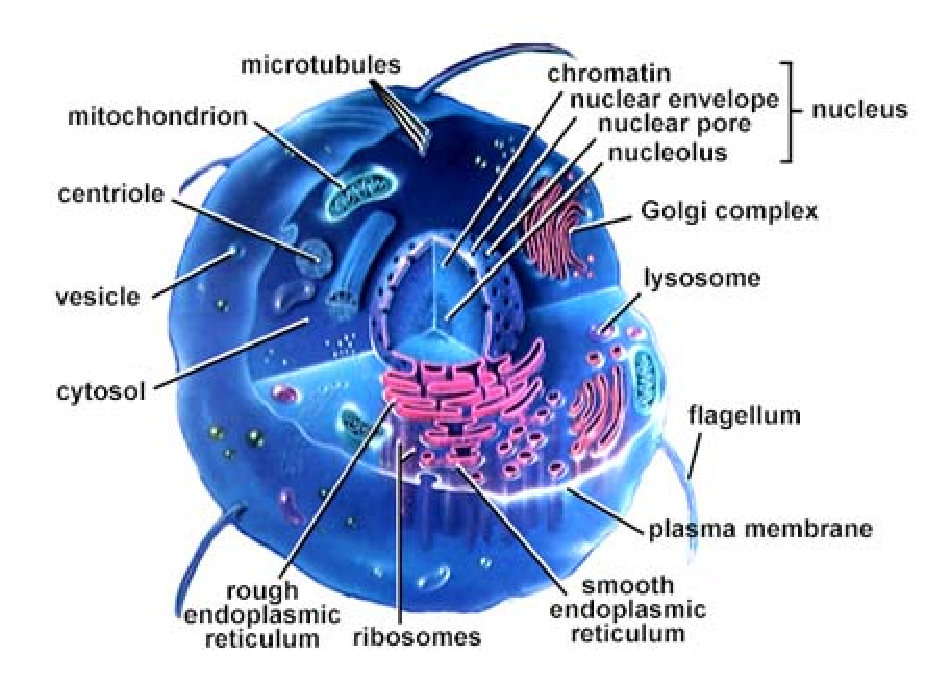
\includegraphics{introduction/eukaryote_cell.eps}}
 \vspace{0.1in}
 \caption{\label{fig:cell}Eukaryote cell}
 \end{center}
 }
 \hfill
 \parbox[b]{0.5 \textwidth}{
 \begin{center}
 \scalebox{0.6}{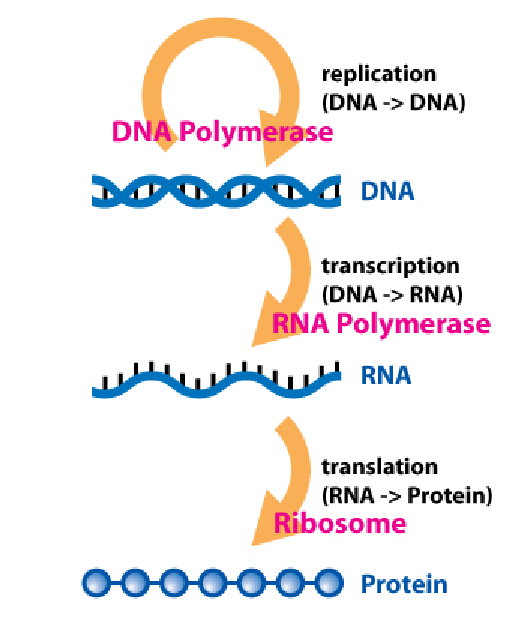
\includegraphics{introduction/central_dogma.eps}}
 \vspace{0.1in}
 \caption{\label{fig:central_dogma}Central dogma of molecular biology: $DNA \longrightarrow RNA \longrightarrow Protein $}
 \end{center}
 }
 \end{figure}

Cells, which are the most fundamental units of life, differ in higher organisms, e.g. multicellular animals and plants, known as \textit{eukaryotes} from those of the less evolved \textit{prokaryotes}, e.g. bacteria, in having a well-defined \textit{nucleus} (see Figure-\ref{fig:cell}\footnote{image taken from online book at \url{http://www.estrellamountain.edu/faculty/farabee/biobk/biobooktoc.html}}) which carries the genetic material. The nucleus is the most prominent structure inside the eukaryotic cell and the genetic information inside it is contained in the form of a \ac{DNA} molecule. \ac{DNA} has a \textit{double-helix} structure formed by two complementary strands, each made up of a sequence of \textit{nucleotides} which are composed of adenine, thymine, cytosine or guanine. 

The central dogma of molecular biology is that the sequence information on the DNA is converted into \ac{RNA} through the process of \textit{transcription}. This sometimes is also referred as \textit{gene expression}. \ac{RNA}, through the process of \textit{translation} is later converted into a sequence of amino acids that results in a \textit{protein} (see Figure-\ref{fig:central_dogma}\footnote{image source: \url{http://en.wikipedia.org/wiki/File:Central\_Dogma\_of\_Molecular\_Biochemistry\_with\_Enzymes.jpg}}). The functional unit on the DNA that codes for an individual protein is known as a \textit{gene}. The sequence of the nucleotides in the double helix within a gene specifies the primary structure of a protein. The complete sequence of nucleotides on the DNA is also referred to as the \textit{DNA sequence}. 
Higher organisms are made up of various different cell types each of which performs a specific role requiring a specific set of gene products. The fascinating fact is that each of these cells contains exactly the same set of genes (DNA) but a different set of gene products. The remarkable diversity among the cells is a result of a precisely controlled mechanism of expression and regulation of a subset of genes in each cell type. 

\begin{figure}[ht]
 \centering
 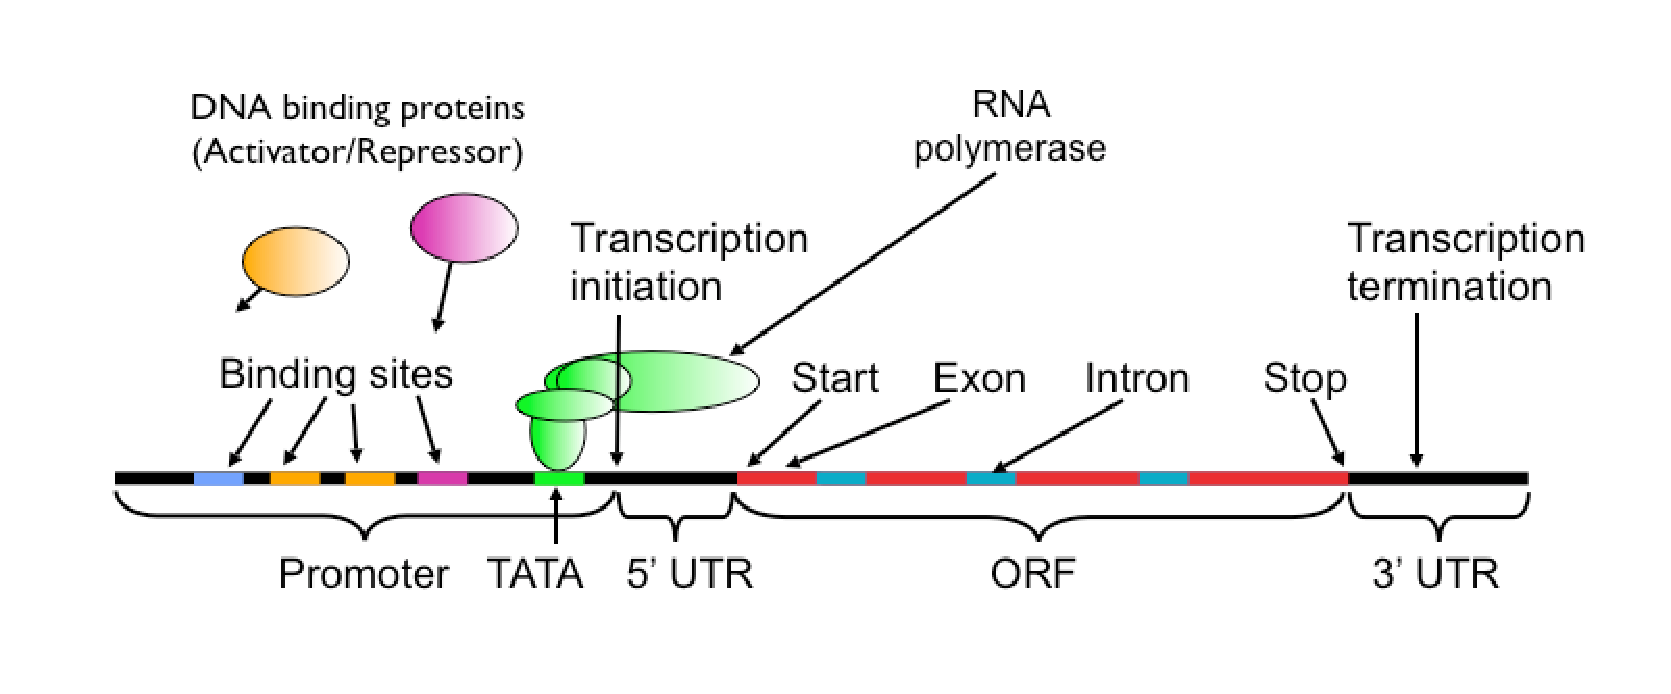
\includegraphics[scale=0.6]{introduction/gene_regulation.eps}
 \caption{Gene regulation}
 \label{fig:gene_regulation}
\end{figure}
The transcription process begins when \acp{TF} are activated by a trans-membrane receptor, leading them to bind to gene regulatory elements and to promote access to the DNA and facilitate the recruitment of RNA polymerase to the transcriptional start site as shown in Figure-\ref{fig:gene_regulation}. The gene regulatory elements of the DNA, also known as \textit{promoter regions}, are situated upstream of the gene at a distance which can vary from a few base pairs to hundreds of base pairs. The regulatory elements contain binding sites for multiple transcription factors allowing each gene to respond to multiple signalling pathways and facilitate fine-tuning of the \acp{mRNA} that are produced. Once the transcription factors are bound on the regulatory elements, they can either promote or inhibit gene expression. In the case of a promoter, the process of transcription starts. A protein called RNA polymerase starts to copy the information contained in the gene into \ac{mRNA}. These \ac{mRNA} molecules, being exact replicas of the gene, contain both \textit{exons} (which will be used in the later process) and \textit{introns} (which will be removed). A process known as \textit{splicing} removes the introns and the remaining \ac{mRNA}, called spliced \ac{mRNA}, is transported out of the nucleus into the cellular material. There it is translated into a polypeptide chain with the help of ribosomes and this chain then folds into a three-dimensional structure known as protein. 

The previous paragraph gives only a partial picture. Since transcription factors themselves are proteins, the same process may regulate them. In fact, there are genes that code just for transcription factors. This process is similar to a feedback loop in which transcription factors are regulated by other transcription factors. A major goal of bioinformatics is to understand how transcription factors affect gene expression and which groups of genes are co-regulated by certain sets of transcription factors. 

\section{Data Sources}\label{bkg:datasources}
Recent technological advances have led to an explosion in both the quantity and types of data being generated. Various observation techniques capture different facets of the cell regulatory process. These are primarily generated by molecular biologists using experimental techniques. Some of the types currently available are:
\begin{itemize}
  \item \ac{mRNA} expression measured using microarrays. 
  \item Whole genome transcription factor binding measured using \ac{ChIP} on chip. 
  \item \ac{TF} binding motifs from the promoter sequences of genes. 
  \item Protein-protein interactions using co-immunoprecipitation and other techniques. 
\end{itemize}

\subsection{Microarrays}
\begin{floatingfigure}[p]{0.45\textwidth}
%\centering
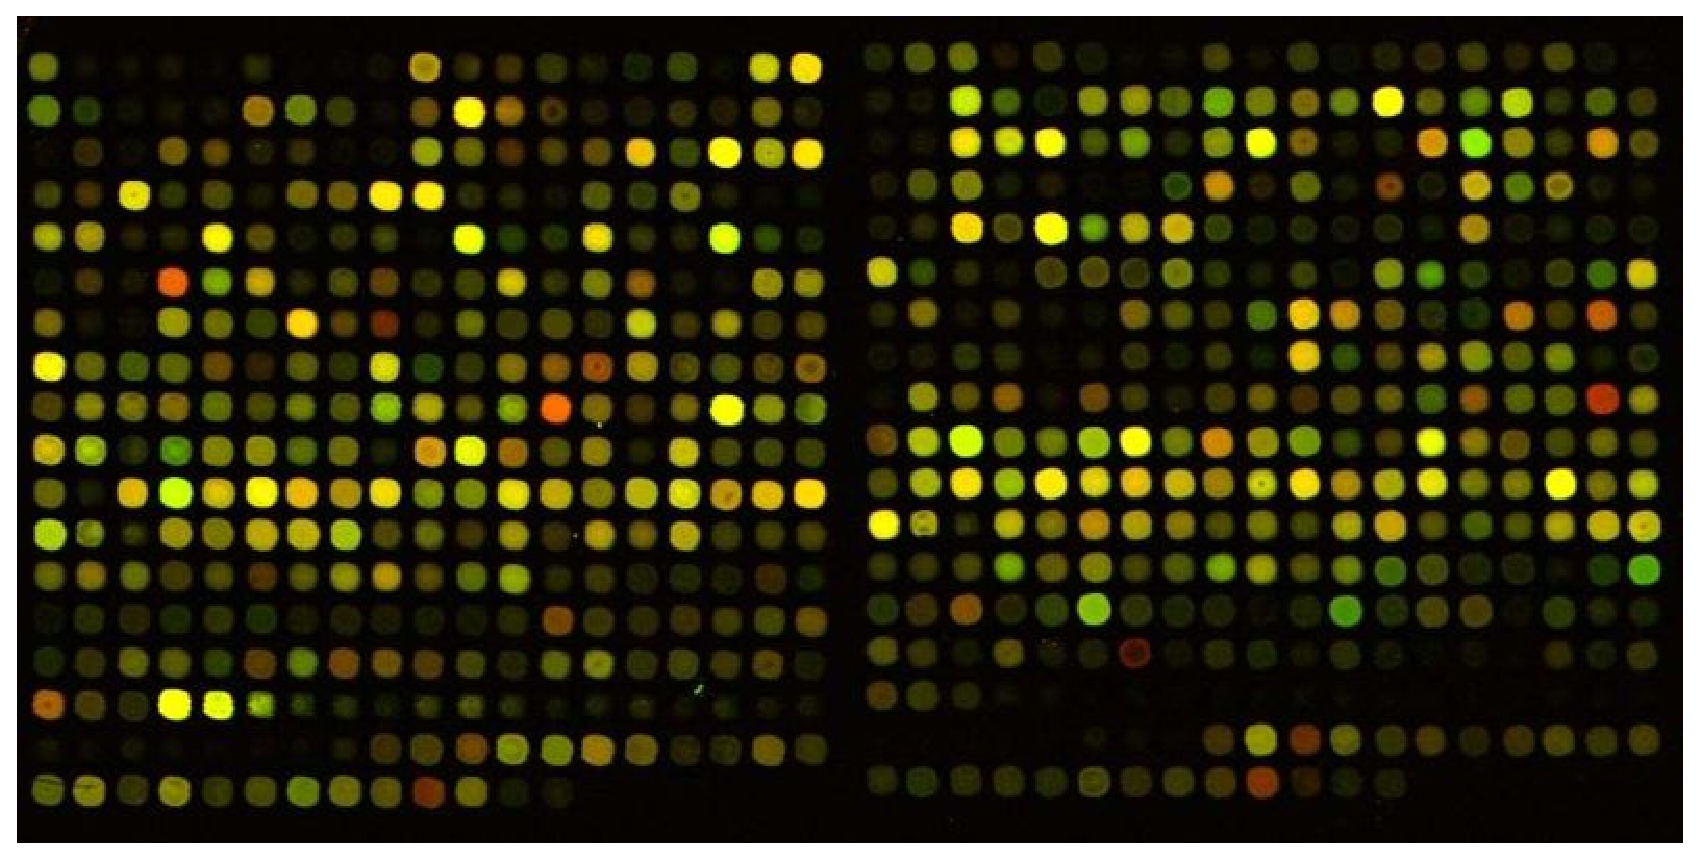
\includegraphics[scale=0.25]{introduction/cdnMicroarray.eps}
\caption{A cross-section of hybridized cDNA microarray}
\label{fig:microarray}
\end{floatingfigure}

One of the most important sources of data related to the transcription process is the genome-wide measurement of \ac{mRNA} expression levels carried out using microarrays. These have received considerable attention in the last six years and various technologies for microarray measurement have been developed \citep{Schulze01navigating}. A microarray allows simultaneous measurement of the expression levels of a large number of genes. It consists of a grid of a large number of microscopic \textit{spots} of DNA oligonucleotides on a silicon chip, each containing a specific DNA sequence. Depending on the specific technique of manufacturing, these are either called \textit{cDNA microarrays} or \textit{oligonucleotide microarrays}. Microarray technology is based on the concept of \textit{hybridization} which means that DNA has complementary strands and given the right conditions, complementary strands will bind to each other. We want to measure \ac{mRNA} content, and since \ac{mRNA} is complementary to the DNA strand from which it was created, it will bind to its complement on the probe. Therefore, each of the spots contain a short section of a gene or other DNA element that we want to study as a probe to \textit{hybridize} a complementary cDNA sample (\ac{mRNA}). Before hybridization, the target is tagged with a fluorescent dye so that after hybridization, the intensity of colour detected by a fluorescence-based detector indicates the abundance of the target.

\textit{Two-channel microarrays} as shown in Figure-\ref{fig:microarray} are hybridized with samples from two conditions, e.g. diseased tissue versus healthy tissue, and are tagged with two different colours. Fluorescent dyes Cy3 (green) and Cy5 (red) are commonly used for tagging these samples. The two coloured cDNA samples are mixed and hybridized to a single microarray that is then scanned. Relative intensities of each colour are then used to identify up-regulated and down-regulated genes. On the other hand, in \textit{single-channel microarrays}, the arrays are designed to give estimates of the absolute levels of gene expression. Therefore, comparison of two conditions requires two separate single-dye hybridizations. 

Similar expression profiles identify genes that may be controlled by a shared regulatory mechanism. Paul Spellman is one of the microarray pioneers who used it to study global expression of genes at various time points in yeast cell cycle \citep{spellman98comprehensive}. He along with some other researchers \citep{gasch00genomicexpn} also studied the response of the yeast genes when subjected to various kinds of stress. Processing microarray data to reduce the errors introduced at various stages is known as \textit{normalization}. \citet{Quackenbush06computational} provides a good overview of the techniques used for normalization and analyzing while \citet{Smythe03Statistical} discuss in detail the statistical issues involved in normalization. 

\subsection{ChIP on chip}

\ac{ChIP} on chip,  also referred to as \textit{ChIP-chip} assay is a technique which allows us to study genome wide binding of transcription factors to the DNA simultaneously. It combines \textit{\ac{ChIP}} with microarray technology (chip) to determine \textit{in vivo} all the regions of interest on the DNA's promoter regions, i.e., where each of the transcription factors bind. \cite{harbison04transcriptional} determined the global genomic occupancy of 203 transcription factors in yeast, which are all known to bind to DNA in the yeast genome. \cite{lee02transcriptional} produced a similar yeast dataset for a smaller number of transcription factors. Both these researchers reported results in the form of a confidence value (statistical P value) of a transcription factor attaching to the promoter region of a gene. The reason behind using statistical techniques was to average the errors in microarray technology and account for multiple cell populations. One of the prominent problems with such approaches is that in order to infer whether a transcription factor attached to the promoter sequence or not, we have to choose an arbitrary artificial threshold of the P-value. 

\subsection{Transcription factor binding motifs}
Transcription factor binding motifs are sequence patterns observed in the intergenic regions of the genome usually located upstream of the genes (promoter region). They are thought to be responsible for allowing access of transcription factors to binding sites which eventually leads to regulation of transcription. While \textit{ChIP-chip} provides \textit{in vivo} evidence of \ac{TF} binding, this is an indirect technique that was used before the advent of \textit{ChIP-chip}. The primary reason for considering this as an information source in the presence of \textit{ChIP-chip} data is that \textit{ChIP-chip} is very noisy and uses evidence from multiple experiments \citep{lee02transcriptional} to report the possibility of a \ac{TF} binding to the promoter region of a gene in the form of a p-value. 

Most of the approaches to identifying these were based on first clustering genes by co-expression, and then looking for common sequences in the upstream regions of the genes located in the same cluster. The upstream sequences are catalogued in the \ac{YPD}, as well as \ac{SCPD} which is dedicated to the curation of yeast genes' promoter sequences \citep{zhu1999scpd}. 

\subsection{Protein-protein interactions}
\begin{floatingfigure}[p]{0.5\textwidth}
%\centering
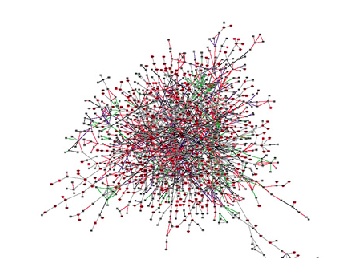
\includegraphics[scale=1.25]{introduction/ppi.eps}
\caption{Protein-protein interactions in yeast}
\label{fig:ppi_yeast}
\end{floatingfigure}
The interactions between proteins is important for many biological functions, e.g. signal transduction, where signals from outside a cell are transmitted to the inside by protein-protein interactions of the signaling molecules. This dataset is important for our study because proteins are gene products and proteins with similar functions and localization are more likely to interact in groups. This was shown by \citet{schwikowski2000protein} where they observed that proteins of known function and cellular location tend to cluster together with 63\% of the interactions between proteins with a common functional assignment and 76\% occurring between proteins found in the same subcellular compartment. Therefore, genes producing interacting proteins are more likely to be co-regulated and have similar functionality. This was verified by \citet{ge01correlation} who provide global evidence that genes with similar expression profiles are more likely to encode interacting proteins. Protein-protein interaction data for yeast is available as a result of advances in technologies like co-immunoprecipitation, mass-spectroscopy and yeast two-hybrid assays. There has been a tremendous growth in this type of data in the recent years. \citet{Gueldener2006MPact} have manually compiled a \ac{PPI} dataset from the literature and published large-scale experiments for yeast which is used as a reference and has been called a gold standard because of its quality and comprehensiveness \citep{yu2004annotation}.
 

\section{Research Goals and Our Approach}
The underlying problem that is addressed results from the nature of the available data. The problem is two fold: firstly, each of the current datasets, e.g. microarrays, DNA-binding, protein-protein interaction and sequence datasets, provide a \textit{partial} and \textit{noisy} picture of the whole process. Hence, we need to integrate them in order to obtain an improved and reliable picture of underlying process. Secondly, the amount of data that is available for each of these types is severely limited. To \textit{learn} good models we need lots of data. Yet, data is only available for few of the experiments of one type. To alleviate this problem many researchers have taken the path of merging available datasets and then learning clusters from it. So, we see that there are two \textit{distinct} types of integration happening, one among \textit{different types} of datasets and the other among datasets of the \textit{same type} but from \textit{different experiments}.

Results are very hard to replicate when the datasets are different even if they result from experiments with the same conditions but done by different experimenters. As clearly stated by \citet{orph02thehuman} there is no single model of regulation and each cell process has evolved its own detailed regulation model. There are certain motifs that can be seen in most of the processes but the actual details of the process are very different from one another. Furthermore, for each underlying motif, the real size of the motif is very different from process to process and geneset to geneset. So, even though many researchers have used this approach of integrating data-sets (both types), its not very clear what the implications on the final results are.

The first part of our research work focuses on \textit{understanding the impact of integration} of the latter type (using datasets of the same type but different experiments) on the global modelling related to the transcriptional gene regulation processes. Most of the algorithms have justified their results \textit{qualitatively} by interpreting their results with the help of biologists. We are interested in studying the \textit{quantitative information overlap} among various datasets and whether our current algorithms are able to leverage the integration of diverse datasets in meaningful \textit{biologically relevant} results. Specifically, we studied the correlation between the theoretical distribution difference among the datasets being merged (using \ac{KL} divergence among distributions) to the functional difference among them (computed using cluster similarity). We also studied how much the functional similarity (in our case, the cluster similarity) varied because of dataset integration as we slowly integrate increasingly diverse datasets. 

The second part of our research deals with proposing a framework and analysis of integrating datasets of different types, e.g. microarray, \textit{ChIP-chip} and PPI datasets. The exact amount of overlap and correlation among functional datasets is unclear \citep{werner2002comparative,kemmeren2002protein}, yet data integration has been shown to increase the accuracy of tasks like gene function prediction compared to single source of data \citep{ge01correlation,gerstein2002proteomics}. For data integration, spectral clustering has been used as our primary tool. The main reason behind this choice is that it is based on computing similarities of variables which results in \textit{affinity} matrices. Similarity computation allows us to normalize diverse datatypes (which were previously considered unintegrable) into a common format (affinity matrices) and then integrate them. Increasingly, biological datasets are non-vectorial, e.g. sequence and PPI data (which is available as a graph). There have been a lot of recent developments in various techniques of similarity computation among these non-vectorial datasets. With this as our foundation, two innovative techniques of integrating these datasets have been proposed.

\subsection{Thesis Scope}
Bioinformatics has grown into a vast field. It is not possible to describe in detail all of the techniques that have been followed or that have been used by the providers of publicly available data. We have not included the details of \textit{within array} normalization techniques of microarray data used by their experimenters and assume that all the microarray data is suitably normalized. 

Even though we have used k-means clustering algorithm, we have not discussed it as it is one of the most well known and elementary techniques. Similarly, we have not discussed the Gene Ontology in great detail. For all these, suitable references have been provided in the thesis.
\section{Thesis Contributions and Publications}
\begin{itemize}
    \item A comprehensive and critical review of research work done in this field has been published as
	\begin{itemize}
	\item Mishra, A. and Gillies, D. (2008). Data integration for regulatory gene module discovery. In Daskalaki, A., editor, \textit{Handbook of Research on Systems Biology Applications in Medicine}. IGI Global, Hershey, PA.
        \end{itemize}	
    \item Issues related to calculation of biological significance of clusters using Gene Ontology has been published as
       \begin{itemize} 
       \item Mishra, A. and Gillies, D. (to be published in 2010). Validation Issues in Regulatory Module Discovery. In: Huma Lodhi and Stephen Muggleton (eds.), Elements of Computational Systems Biology, John Wiley \& Sons, Inc. ISBN: 0470180935.
       \end{itemize}
    \item An empirical technique to calculate the functional similarity of datasets using the concept of cluster similarity has been developed. We propose this can be used as an index for dataset similarity after showing a very high correlation with underlying data distribution differences. We have also demonstrated that dataset integration should only be done by first choosing similar datasets, otherwise the signals present in the datasets could be overwhelmed by noise. Part of this work published as
	\begin{itemize}
	    \item Mishra, A. and Gillies, D. (2007). Effect of microarray data heterogeneity on regulatory gene module discovery. \textit{BMC Systems Biology}, 1(Suppl 1):S2
	\end{itemize}
    \item A semi-supervised spectral clustering technique to integrate two datasets where one is acting as a source of supervision on the clustering of the other has been developed. We validated the results using Gene Ontology.\nocite{mishra2007data,mishra2008Semisup,mishra2007elements} Part of this work published as
	\begin{itemize}
    		\item Mishra, A. and Gillies, D. (2008). Semi supervised spectral clustering for regulatory module discovery. In \textit{Data Integration in the Life Sciences}, pages 192-203.
 	\end{itemize}
    \item A principled technique to integrate two diverse datasets where no evidence is available regarding their individual weights (importance) has been developed using the principle of maximum entropy. We validated the results after spectral clustering of the integrated matrix using Gene Ontology.
    \item Modular and reusable software implementations of all the techniques has been developed using python\footnote{a popular programming language with efficient Linear Algebra library} and R\footnote{a software environment for statistical computing}.	
\end{itemize}

\section{Thesis Outline}
The outline of this thesis is as follows. In Chapter-2, we present a critical literature review related to the evolution of the research related to transcriptional regulatory networks and modules. Even though this field is relatively new, the amount of research done is enormous because of increasing focus and funding. This chapter tries to tie together all the past efforts into a coherent story. 

In Chapter-3, we study the effect of \textit{integrating increasingly diverse microarray datasets}. For functional similarity, we compute the cluster similarity among datasets using modified Rand's index. To estimate the theoretical difference between the underlying distributions of individual datasets, we use the \ac{KL} divergence. Finally, we study the correlation between the two measures (functional and theoretical).

In Chapter-4, we start with a discussion of spectral clustering and its theoretical foundations. In order to integrate microarray datasets with other datasets e.g., PPI and DNA-binding datasets, we propose a semi-supervised spectral clustering technique. We apply this technique on two of the popular yeast microarray datasets and evaluate the results of integration using the Gene Ontology. 

While the semi-supervised algorithm is heuristic in combining separate evidence of similarity, in Chapter-5, we propose a more principled approach to integration of similarity matrices. We merge similarity matrices derived from various datasets (microarray, PPI and DNA-binding) using the principle of maximum entropy \citep{jaynes57maxent} and analyze the results.

Finally, Chapter-6 concludes this thesis with remarks about the drawbacks and challenges faced in our approach. It details where the field is heading and what would be the future challenges. We also discuss the scope and direction of extending the current work in future. 
